\documentclass{beamer}

\usetheme{simple}

\usepackage{lmodern}
\usepackage[scale=2]{ccicons}

\usepackage{bussproofs}

\usepackage{mathpartir}

\usepackage{tikz}
\usetikzlibrary{arrows,positioning}
\tikzset{
    %Define standard arrow tip
    >=stealth',
    %Define style for boxes
    punkt/.style={
           rectangle,
           rounded corners,
           draw=black,
           text width=7.5em,
           minimum height=2em,
           text centered},
    % Define arrow style
    pil/.style={
           ->,
           thick,
           shorten <=2pt,
           shorten >=2pt,}
}



\title{On the Lambek Calculus with an Exchange Modality}
\subtitle{}
\date{July 5, 2018}
\author{Jiaming Jiang$^1$, Harley Eades III$^2$, Valeria de Paiva$^3$}
\institute{$^1$North Carolina State University; $^2$Augusta University; $^3$Nuance Communications}

\begin{document}

\maketitle


%--------------------------------------------------
% (Temporary slide)
%--------------------------------------------------
\begin{frame}{Outline 1}
\begin{itemize}
\item Objective: To isolate exchange using a modality, $eA$, in the same
      way that the of-course modality of linear logic, $!A$, isolates
      weakening and contraction. \\
      $\Rightarrow$ \\
      To add an exchange modality, $eA$, such that one can show
      that $eA\otimes eB\multimap eB\otimes eA$ holds
\item Motivation: In process calculi: $A\otimes B$ as both processes in
      parallel, $A\triangleright B$ as first runs process $A$ and then
      process $B$ \\
      \textit{A note on notation}
\item Basic Approach: generalize LNL model
\item Introduction to LNL model: with diagram
\item How to generalize LNL model to monoidal categories
\end{itemize}
\end{frame}



%--------------------------------------------------
% (Temporary slide)
%--------------------------------------------------
\begin{frame}{Outline 2}
\begin{itemize}
\item CNL Logic:
      \begin{enumerate}
      \item Introduce the term CNC logic
      \item Brief description of CNC logic: abstracts Benton's LNL logic by
            removing the existince of the exchange structural rule
      \item A diagram for Benton's LNL logic, and LNL categorical model
      \item A diagram for CNC logic and the categorical model, compare with 
            LNL
      \end{enumerate}
\item Previous approach in isolating exchange
      \begin{itemize}
      \item Brief introduction to the inference rules of reference 8
      \item Limitations of the approach
      \end{itemize}
\item More detailed introduction to CNC logic: include some example rules
\item One slide for other results: $\beta$-reductions, commuting
      conversions, sequent calculus, natural deduction, etc
\item One slide for dialectica model
\item Conclusion ``take away'' slide
\end{itemize}
\end{frame}


%--------------------------------------------------
% 1.a. Objective (a)
%--------------------------------------------------
\begin{frame}{Objective}

Linear logic uses the of-course modality, $!A$, to isolate
\textit{weakening} and \textit{contraction}:
$$\mbox{Weakening: }!X \rightarrow I$$
$$\mbox{Contraction: }!X \rightarrow !X \otimes !X$$

\invisible{
\begin{block}{}
To isolate \textit{exchange} using a modality, $eA$:
$$eA\otimes eB\multimap eB\otimes eA$$.
\end{block}
}

\end{frame}


%--------------------------------------------------
% 1.b. Objective (b)
%--------------------------------------------------
\begin{frame}{Objective}

Linear logic uses the of-course modality, $!A$, to isolate
\textit{weakening} and \textit{contraction}:
$$\mbox{Weakening: }!X \rightarrow I$$
$$\mbox{Contraction: }!X \rightarrow !X \otimes !X$$

\begin{block}{Exchange Modality}
To isolate \textit{exchange} using a modality, $eA$:
\begin{gather*}
eA\otimes eB\multimap eB\otimes eA
\end{gather*}
\end{block}

\end{frame}


%--------------------------------------------------
% 2. Motivation
%--------------------------------------------------
\begin{frame}{Motivation}

In process calculi, to model sequential composition of processes:

\begin{columns}
\column{.4\textwidth}
  \begin{block}{$A\otimes B$}
  \begin{itemize}
  \item Commutative tensor product
  \item Processes $A$ and $B$ run in parallel
  \end{itemize}
  \end{block}
\column{.4\textwidth}
  \begin{block}{$A\triangleright B$}
  \begin{itemize}
  \item Non-commutative tensor product
  \item Process $A$ runs first, then process $B$
  \end{itemize}
  \end{block}
\end{columns}

\end{frame}

%--------------------------------------------------
% 3. Basic Approach
%--------------------------------------------------
\begin{frame}{Basic Approach}

Abstract Benton's Linear/Non-Linear (LNL) model:
\begin{itemize}
\item Remove the exchange structural rule
\item Two logics:
      \begin{itemize}
      \item Intuitionistic linear logic
      \item Lambek Calculus
      \end{itemize}
\end{itemize}

\end{frame}


%--------------------------------------------------
% 4. LNL Model
%--------------------------------------------------
\begin{frame}{Linear/Non-Linear Model}

A symmetric monoidal adjunction $F\dashv G$:

\begin{center}
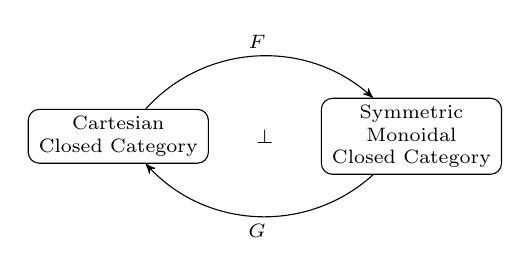
\begin{tikzpicture}[node distance=0.5cm, auto,]
  \scriptsize
  \node (adjoint) {$\perp$};
  \node[punkt,left=of adjoint] (ccc) {Cartesian Closed Category};
  \node[punkt,right=of adjoint] (smcc) {Symmetric Monoidal Closed Category}
    edge[<-,bend right=45] node[above] {$F$} (ccc)
    edge[->,bend left=45] node[auto] {$G$} (ccc);
\end{tikzpicture}
\end{center}

\end{frame}


%--------------------------------------------------
% 5.a. CNC Model (a)
%--------------------------------------------------
\begin{frame}{Commutative/Non-Commutative Model}

\begin{center}
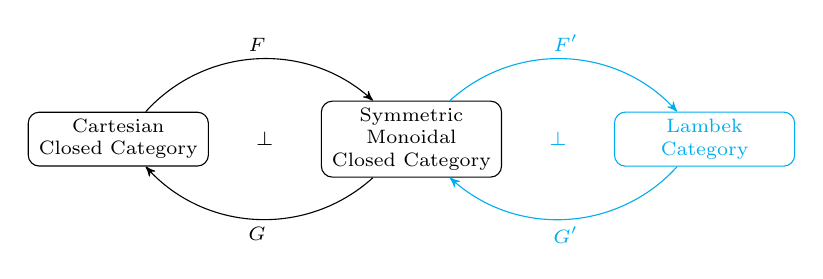
\begin{tikzpicture}[node distance=0.5cm, auto,]
  \scriptsize
  \node (adjoint1) {$\perp$};
  \node[punkt,left=of adjoint1] (ccc) {Cartesian Closed Category};
  \node[punkt,right=of adjoint1] (smcc) {Symmetric Monoidal Closed Category}
    edge[<-,bend right=45] node[above] {$F$} (ccc)
    edge[->,bend left=45] node[auto] {$G$} (ccc);
  \node[right=of smcc,cyan] (adjoint2) {$\perp$};
  \node[punkt,right=of adjoint2,cyan] (lambek) {Lambek Category}
    edge[<-,bend right=45,cyan] node[above] {$F'$} (smcc)
    edge[->,bend left=45,cyan] node[auto] {$G'$} (smcc);
\end{tikzpicture}
\end{center}

\end{frame}


%--------------------------------------------------
% 5.b. CNC Model (b)
%--------------------------------------------------
\begin{frame}{Commutative/Non-Commutative Model}

A monoidal adjunction $F\dashv G$:

\begin{center}
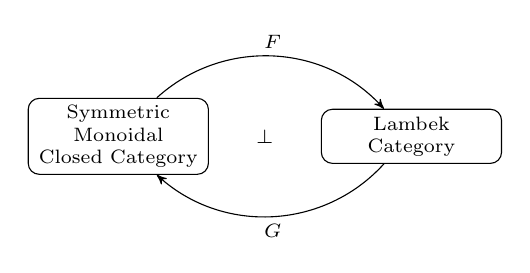
\begin{tikzpicture}[node distance=0.5cm, auto,]
  \scriptsize
  \node (adjoint) {$\perp$};
  \node[punkt,left=of adjoint] (smcc) {Symmetric Monoidal Closed Category};
  \node[punkt,right=of adjoint] (lambek) {Lambek Category}
    edge[<-,bend right=45] node[above] {$F$} (smcc)
    edge[->,bend left=45] node[auto] {$G$} (smcc);
\end{tikzpicture}
\end{center}

\end{frame}


%--------------------------------------------------
% 6. CNC Logic
%--------------------------------------------------
\begin{frame}{CNC Logic}

(Add ILL to the left of the diagram of CNC model, \\
add Lambek calculus to the right)

\end{frame}



\end{document}


















